\chapter{تضاعف DNA}\label{ch:g11:dna-replication}

ينتج نقي عظمك كل يوم مئتي مليار كرية حمراء جديدة، وتستبدل بطانة معيك
نفسها كل بضعة أيام، وتتلقى كل \omterm{def:g10:cells-common-unit:cell}{خلية} من تلك \omterm{def:g10:cells-common-unit:cell}{الخلايا} الجديدة نسخة كاملة
من المترين من \omterm{def:g10:universal-dna:information}{DNA} اللذين وصفتهما الفصول السابقة بنص \omterm{def:g10:cells-common-unit:cell}{الخلية}. فنسخ ثلاثة
مليارات حرف، من دون أصل يراجع، في بضع ساعات، بأخطاء أقل مما يرتكبه
طابع محترف في صفحة: كيف يجري ذلك؟ خُمّن الجواب من بنية الجزيء نفسه سنة
1953، وأثبتته بعد خمس سنوات واحدة من أنيق التجارب في البيولوجيا.

\section{مشكلة النسخ}

\begin{definition}[التضاعف]\label{def:g11:dna-replication:replication}
\emph{تضاعف DNA}\index{تضاعف DNA} هو العملية التي تصنع بها \omterm{def:g10:cells-common-unit:cell}{الخلية}، من
جزيء \omterm{def:g10:universal-dna:information}{DNA} مزدوج الشريط واحد، جزيئين مطابقين له ومتطابقين. وهو يجري في
مرحلة محددة من الدورة الخلوية، هي \emph{المرحلة S}
(\cref{ch:g11:cell-cycle-mitosis})، تتضاعف فيها كمية \omterm{def:g10:universal-dna:information}{DNA} في \omterm{def:g10:cells-common-unit:organelle}{النواة}.
\end{definition}

\begin{proposition}[مبدأ الأصل]\label{prop:g11:dna-replication:template}
لما كان شريطا جزيء \omterm{def:g10:universal-dna:information}{DNA} متممين --- A تواجه T، وG تواجه C --- حمل كل
شريط كل المعلومة اللازمة لإعادة بناء الآخر. ومن ثم يجري التضاعف بفصل
الشريطين واستعمال كل منهما \emph{أصلًا} يركّب عليه شريط متمم جديد،
نوكليوتيدًا نوكليوتيدًا.
\end{proposition}
\admitted

\begin{example}[ثلاث نتائج ممكنة]\label{ex:g11:dna-replication:models}
انطلاقًا من مبدأ الأصل، اقترحت في الخمسينيات ثلاث طرق لتوزيع الشريطين
القديم والجديد:
\begin{itemize}
  \item \emph{نصف محافظ}: يحتفظ كل جزيء بنت بشريط قديم ويأخذ شريطًا
        جديدًا؛
  \item \emph{محافظ}: يحفظ الجزيء الأصلي كاملًا ويبنى بجانبه شريط
        مزدوج جديد كله؛
  \item \emph{مبدد}: تتناوب القطع القديمة والجديدة على طول كل شريط في
        البنتين.
\end{itemize}
والثلاثة لا تميز بالنظر؛ وإنما تميز بالوزن.
\end{example}

\section{تجربة ميزلسون وستال}

\begin{proposition}[التضاعف نصف محافظ]\label{prop:g11:dna-replication:semiconservative}
يحوي كل جزيء \omterm{def:g10:universal-dna:information}{DNA} بنت شريطًا من الجزيء الأب وشريطًا مركبًا حديثًا.
\end{proposition}
\begin{proof}[شواهد]
ربّى ميزلسون وستال (1958) بكتيريا أجيالًا كثيرة في وسط نيتروجينه
الوحيد هو النظير الثقيل $^{15}$N، حتى صار \omterm{def:g10:universal-dna:information}{DNA} فيها كله ثقيلًا. ثم
نقلاها إلى وسط $^{14}$N العادي وأخذا عينات من المزرعة بعد كل جيل (كل
عشرين دقيقة). وكان \omterm{def:g10:universal-dna:information}{DNA} المستخلص من كل عينة يدوَّر ساعات طويلة في محلول
ملحي كثيف، يطفو فيه الجزيء عند المستوى الموافق لكثافته هو، ثم يصوَّر
تحت الأشعة فوق البنفسجية: فيكوّن \omterm{def:g10:universal-dna:information}{DNA} الثقيل والخفيف نطاقين تفصل
بينهما مسافة قابلة للقياس. والنتائج: قبل النقل، نطاق ثقيل واحد؛ وبعد
جيل واحد، نطاق واحد في منتصف المسافة بين الثقيل والخفيف بالضبط ---
فكل جزيء هجين؛ وبعد جيلين، نطاقان متساويا الشدة، أحدهما هجين والآخر
خفيف؛ وبعد ثلاثة، النطاق الخفيف ثلاثة أمثال الهجين. والنموذج المحافظ
يتنبأ بنطاق ثقيل وآخر خفيف عند الجيل الأول، ولا هجين قط؛ والنموذج
المبدد يتنبأ بنطاق واحد يخف كل جيل، ولا ينقسم إلى اثنين قط. فما من
نموذج يعطي نطاقًا هجينًا واحدًا، ثم هجينًا وخفيفًا بالنسب المشاهدة،
إلا النموذج النصف المحافظ.
\end{proof}

\begin{omfigure}
\begin{tikzpicture}[font=\small]
  \tikzset{tube/.style={draw, thick, rounded corners=6pt, minimum width=1.3cm, minimum height=3.6cm}}
  \foreach \x/\g in {0/{الجيل 0}, 3/{الجيل 1}, 6/{الجيل 2}, 9/{الجيل 3}} {
    \node[tube] (t\x) at (\x,0) {};
    \node[anchor=north, align=center] at (\x,-1.95) {\g};
  }
  \draw[dashed, gray] (-1.0,1.2) -- (10.6,1.2) node[right, gray] {خفيف};
  \draw[dashed, gray] (-1.0,0.0) -- (10.6,0.0) node[right, gray] {هجين};
  \draw[dashed, gray] (-1.0,-1.2) -- (10.6,-1.2) node[right, gray] {ثقيل};
  % bands: width encodes intensity
  \fill[omDef] (-0.55,-1.28) rectangle (0.55,-1.12);
  \fill[omDef] (2.45,-0.08) rectangle (3.55,0.08);
  \fill[omDef] (5.45,-0.06) rectangle (6.55,0.06);
  \fill[omDef] (5.45,1.14) rectangle (6.55,1.26);
  \fill[omDef] (8.45,-0.03) rectangle (9.55,0.03);
  \fill[omDef] (8.45,1.11) rectangle (9.55,1.29);
  \node[anchor=south, align=center] at (4.5,2.0) {نطاقات DNA بعد التدوير في تدرج كثافة};
\end{tikzpicture}

{\small نتيجة ميزلسون وستال. \omterm{def:g10:universal-dna:information}{DNA} ثقيل قبل النقل؛ ونطاق هجين واحد بعد
جيل في الوسط الخفيف؛ وهجين وخفيف بمقدارين متساويين بعد جيلين؛ وخفيف
ثلاثة أمثال الهجين بعد ثلاثة. وسمك النطاق يمثل كمية \omterm{def:g10:universal-dna:information}{DNA}.}
\end{omfigure}

\begin{omfigure}
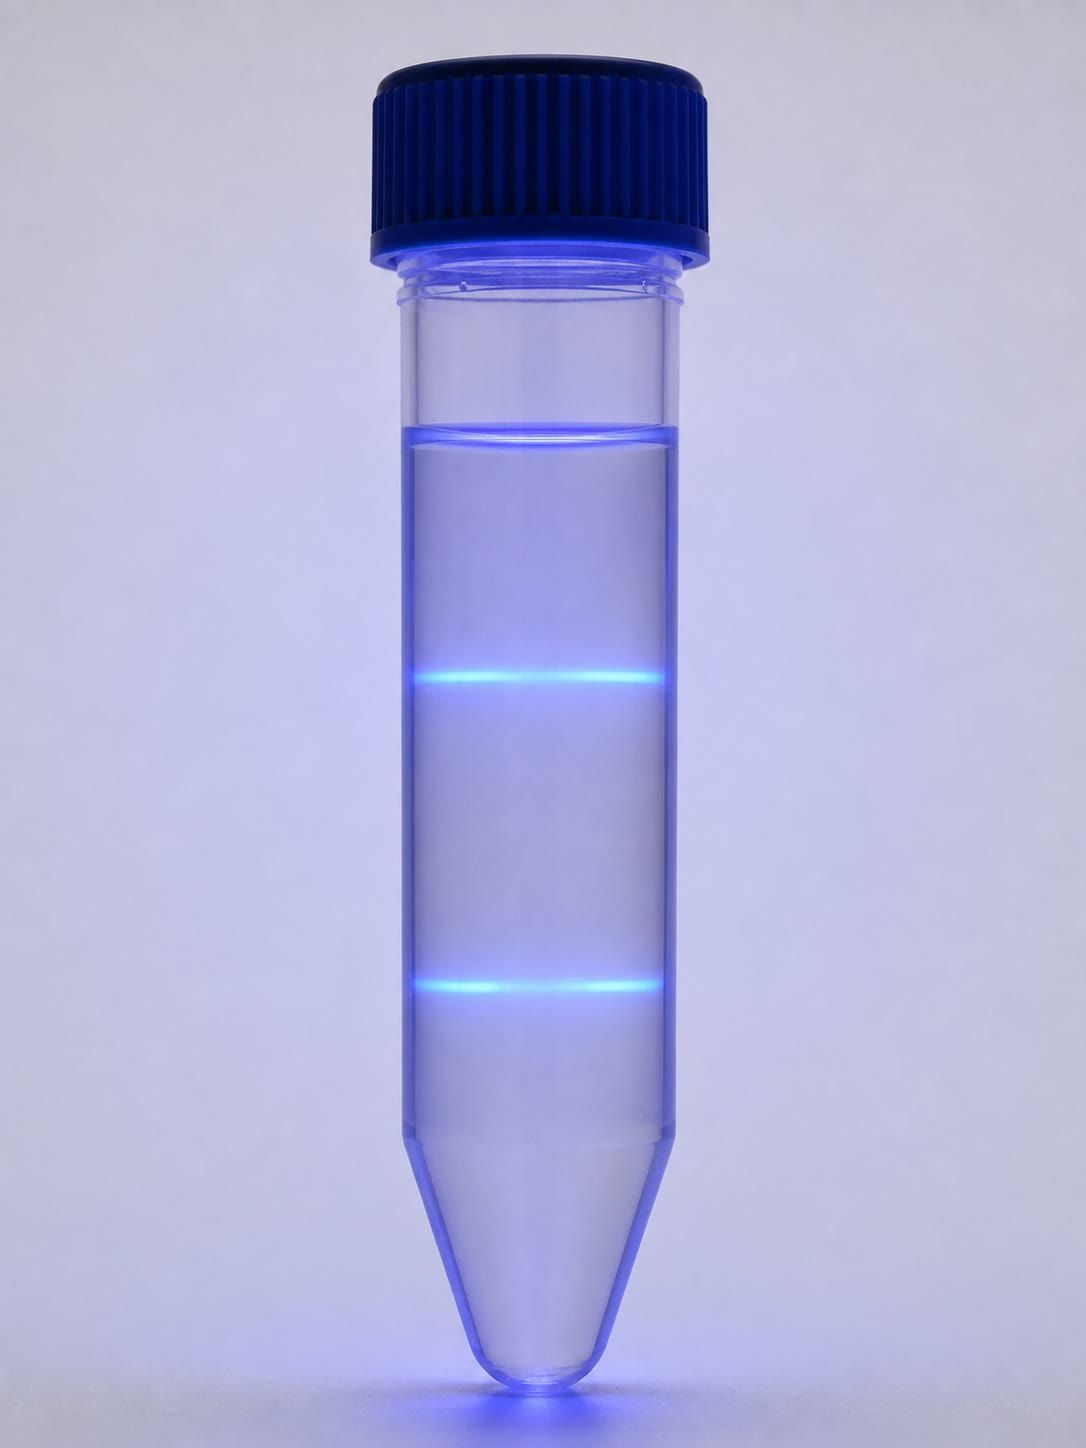
\includegraphics[width=0.3\linewidth]{images/book2/ai/g11-replication-centrifuge-tube.jpg}

{\small أنبوب طرد مركزي تحت الأشعة فوق البنفسجية: جزيئات \omterm{def:g10:universal-dna:information}{DNA} من
كثافتين قد طفت إلى مستويين من التدرج الملحي وتظهر نطاقين. فموضعهما
يقيس كثافتهما؛ وسطوعهما يقيس مقدارهما.}
\end{omfigure}

\begin{example}[التنبؤ بالجيل الرابع]\label{ex:g11:dna-replication:fourth}
بعد $n$ جيلًا في وسط خفيف، يظل الشريطان الثقيلان الأصليان موجودين،
واحد في كل من جزيئين هجينين؛ وكل جزيء آخر خفيف كله. فمن أصل $2^n$
جزيء، 2 هجينان و$2^n - 2$ خفيفة: فعند الجيل 4، 2 هجينان مقابل 14
خفيفًا --- أي نطاق خفيف سبعة أمثال الهجين، والنطاق الهجين لا يختفي
قط، بل يخفت فقط. فالشريطان الأصليان خالدان في الواقع.
\end{example}

\section{الآلة}

\begin{proposition}[شوكات التضاعف]\label{prop:g11:dna-replication:forks}
يبدأ التضاعف عند مواضع محددة، هي \emph{المنشآت}، حيث يشد الشريطان
متباعدين في فقاعة. وعند كل حافة من الفقاعة تتقدم \emph{شوكة
تضاعف}\index{شوكة تضاعف}: فينتقل \omterm{def:g10:cell-metabolism:metabolism}{إنزيم}، هو \emph{بوليميراز
DNA}\index{بوليميراز DNA}، على كل شريط مفتوح ويضيف، واحدًا واحدًا،
\omterm{def:g10:universal-dna:nucleotide}{النوكليوتيدات} المتممة له، فيسلسلها في الشريط الجديد. وشوكتا الفقاعة
تسيران في اتجاهين متعاكسين حتى تلقيا شوكتي الفقاعتين المجاورتين؛
وللصبغي الجرثومي، وهو حلقة واحدة، منشأ واحد وشوكتان؛ أما \omterm{def:g10:universal-dna:information}{الصبغي} البشري
فله آلاف المنشآت تعمل في آن واحد.
\end{proposition}
\admitted

\begin{omfigure}
\begin{tikzpicture}[font=\small, >=Stealth, line cap=round]
  % parent strands
  \draw[very thick, omDef] (0,0.5) -- (4,0.5);
  \draw[very thick, omDef] (0,-0.5) -- (4,-0.5);
  \draw[very thick, omDef] (4,0.5) .. controls (5.5,0.5) and (6,1.4) .. (8.5,1.6);
  \draw[very thick, omDef] (4,-0.5) .. controls (5.5,-0.5) and (6,-1.4) .. (8.5,-1.6);
  % new strands
  \draw[very thick, omThm] (4.4,0.35) .. controls (5.6,0.4) and (6,1.0) .. (8.5,1.2);
  \draw[very thick, omThm] (4.4,-0.35) .. controls (5.6,-0.4) and (6,-1.0) .. (8.5,-1.2);
  % base pair rungs (parent)
  \foreach \x in {0.3,0.7,...,3.9} \draw[gray] (\x,0.5) -- (\x,-0.5);
  % rungs in daughter helices
  \foreach \t in {0.15,0.3,...,0.95} {
    \draw[gray] ({4+4.5*\t},{0.5+1.1*\t*\t+0.0}) -- ({4+4.5*\t},{0.35+0.85*\t*\t});
    \draw[gray] ({4+4.5*\t},{-0.5-1.1*\t*\t}) -- ({4+4.5*\t},{-0.35-0.85*\t*\t});
  }
  % polymerases
  \node[draw, fill=omProp!35, circle, minimum size=0.55cm, inner sep=0] (p1) at (6.6,0.95) {};
  \node[draw, fill=omProp!35, circle, minimum size=0.55cm, inner sep=0] (p2) at (6.6,-0.95) {};
  \node[anchor=south, align=center] at (6.6,2.0) {بوليميراز DNA};
  \draw[->] (6.6,1.95) -- (p1.north);
  \draw[->] (6.6,-1.95) -- (p2.south);
  \node[anchor=north, align=center] at (6.6,-2.05) {بوليميراز DNA};
  % labels
  \node[anchor=east, omDef, align=right] at (-0.15,0) {الشريط المزدوج\\ الأب};
  \node[anchor=west, align=left] at (8.7,1.4) {البنت 1};
  \node[anchor=west, align=left] at (8.7,-1.4) {البنت 2};
  \draw[->, thick] (2.0,-1.5) -- (3.9,-1.5) node[midway, below] {الشوكة تتقدم};
  \node[omDef, anchor=south west] at (0.1,0.6) {شريط قديم};
  \node[omThm, anchor=north west] at (5.6,-0.05) {شريط جديد};
\end{tikzpicture}

{\small \omterm{prop:g11:dna-replication:forks}{شوكة تضاعف}. الشريطان الأبوان (بالأزرق) ينفصلان؛ وعلى كل منهما
يبني \omterm{prop:g11:dna-replication:forks}{بوليميراز DNA} شريطًا متممًا جديدًا (بالأحمر). ووراء الشوكة شريطان
مزدوجان، في كل منهما شريط قديم وشريط جديد.}
\end{omfigure}

\begin{example}[السرعة والسلّم]\label{ex:g11:dna-replication:speed}
تضيف الشوكة الجرثومية نحو 1000 \omterm{def:g10:universal-dna:nucleotide}{نوكليوتيد} في الثانية؛ والشوكة البشرية
نحو 50. \omterm{def:g10:universal-dna:information}{وصبغي} \emph{E.~coli}، وفيه $\num{4.6e6}$ زوج قواعد، تنسخه
شوكتان من منشأ واحد في $\num{4.6e6}/(2 \times
1000) \approx \qty{2300}{s}$، أي نحو 40 دقيقة --- وهي مدة الدورة
الخلوية للبكتيريا في وسط غني. أما \omterm{def:g10:cells-common-unit:cell}{الخلية} البشرية، وعليها نسخ
$\num{6.4e9}$ زوج قواعد في مرحلة S تدوم نحو 8 ساعات، فتحتاج إلى آلاف
منشآتها: فشوكة واحدة كانت لتستغرق أكثر من سنتين.
\end{example}

\begin{omfigure}
\begin{tikzpicture}[font=\small, >=Stealth]
  \foreach \y/\lab in {0/{بداية المرحلة S}, -1.4/{لاحقًا}, -2.8/{نهاية المرحلة S}} {
    \node[anchor=east] at (-0.3,\y) {\lab};
  }
  % row 1: single line with origins marked
  \draw[very thick, omDef] (0,0) -- (10,0);
  \foreach \x in {1.5,4,6.5,9} \fill[omThm] (\x,0) circle (2pt);
  \node[anchor=west, font=\scriptsize] at (10.1,0) {المنشآت};
  % row 2: bubbles
  \draw[very thick, omDef] (0,-1.4) -- (10,-1.4);
  \foreach \x/\w in {1.5/0.7, 4/0.9, 6.5/0.6, 9/0.5} {
    \draw[very thick, omDef, fill=white] (\x-\w,-1.4) .. controls (\x-\w/2,-1.05) and (\x+\w/2,-1.05) .. (\x+\w,-1.4)
      .. controls (\x+\w/2,-1.75) and (\x-\w/2,-1.75) .. (\x-\w,-1.4);
    \draw[very thick, omThm] (\x-\w+0.05,-1.4) .. controls (\x-\w/2,-1.15) and (\x+\w/2,-1.15) .. (\x+\w-0.05,-1.4);
    \draw[very thick, omThm] (\x-\w+0.05,-1.4) .. controls (\x-\w/2,-1.65) and (\x+\w/2,-1.65) .. (\x+\w-0.05,-1.4);
    \draw[->, thick] (\x-\w-0.05,-1.4) -- (\x-\w-0.45,-1.4);
    \draw[->, thick] (\x+\w+0.05,-1.4) -- (\x+\w+0.45,-1.4);
  }
  % row 3: two full molecules
  \draw[very thick, omDef] (0,-2.65) -- (10,-2.65);
  \draw[very thick, omThm] (0,-2.8) -- (10,-2.8);
  \draw[very thick, omThm] (0,-3.0) -- (10,-3.0);
  \draw[very thick, omDef] (0,-3.15) -- (10,-3.15);
  \node[anchor=west, font=\scriptsize, align=left] at (10.1,-2.9) {نسختان};
\end{tikzpicture}

{\small تضاعف \omterm{def:g10:universal-dna:information}{صبغي} طويل من منشآت كثيرة. تنفتح الفقاعات عند المنشآت،
ولكل منها شوكتان تتباعدان؛ فتنمو وتتلاقى وتندمج، تاركةً شريطين مزدوجين
كاملين، كل منهما نصفه قديم (بالأزرق) ونصفه جديد (بالأحمر).}
\end{omfigure}

\begin{proposition}[الأمانة]\label{prop:g11:dna-replication:fidelity}
\omterm{prop:g11:dna-replication:forks}{بوليميراز DNA} يزاوج \omterm{def:g10:universal-dna:nucleotide}{النوكليوتيد} الخطأ نحو مرة في كل $10^5$؛ وهو يتحقق
من كل \omterm{def:g10:universal-dna:nucleotide}{نوكليوتيد} وهو يضيفه ويزيل معظم عدم التطابق في الحال، وإنزيمات
أخرى تصحح معظم الباقي وراء الشوكة مباشرة. ونسبة الخطأ النهائية نحو
واحد في كل $10^9$ \omterm{def:g10:universal-dna:nucleotide}{نوكليوتيد}: \omterm{def:g10:cells-common-unit:cell}{فالخلية} البشرية، وهي تنسخ $\num{6.4e9}$
\omterm{def:g10:universal-dna:nucleotide}{نوكليوتيد}، ترتكب وسطيًا نحو نصف دزينة من الأخطاء في كل انقسام. وما
يفلت منها \emph{طفرات}، وهي موضوع \cref{ch:g11:mutations}.
\end{proposition}
\admitted

\begin{method}[حسابات التضاعف]\label{met:g11:dna-replication:calc}
\begin{enumerate}
  \item \emph{الزمن}: الطول المراد نسخه (بأزواج القواعد) مقسومًا على
        السرعة الكلية لكل الشوكات العاملة (عدد الشوكات $\times$
        \omterm{def:g10:universal-dna:nucleotide}{النوكليوتيدات} في الثانية للشوكة).
  \item \emph{المنشآت اللازمة}: الطول الكلي مقسومًا على ما يستطيع
        منشأ واحد (شوكتان) نسخه في الزمن المتاح.
  \item \emph{الأخطاء}: \omterm{def:g10:universal-dna:nucleotide}{النوكليوتيدات} المنسوخة $\times$ نسبة الخطأ؛
        وتذكر أن \omterm{def:g10:cells-common-unit:cell}{الخلية} تنسخ الشريطين معًا، أي ضعف عدد أزواج القواعد.
  \item \emph{تجارب النظائر}: تتبّع الشريطين الأصليين؛ فبعد $n$ جيلًا
        يقعان في جزيئين هجينين من أصل $2^n$.
\end{enumerate}
\end{method}

\begin{remark}[لماذا تتوافق البنية والآلية]\label{rem:g11:dna-replication:fit}
ختم واطسون وكريك مقالتهما سنة 1953 بملاحظة أن الازدواج «يوحي في الحال
بآلية نسخ ممكنة». وبيّن ميزلسون وستال أنها الآلية الفعلية؛ ثم بيّن علم
الإنزيمات الذي تلاهما كيف تعمل. وهي من الحالات النادرة في البيولوجيا
التي أملى فيها شكل جزيء، رئي مرة واحدة، العمليةَ التي تستعمله.
\end{remark}

\section{تمارين}

\begin{exercise}[$\star$]\label{exo:g11:dna-replication:1}
اذكر مبدأ الأصل وفسّر لماذا يتوقف على \omterm{prop:g10:universal-dna:helix}{التتام}.
\end{exercise}

\begin{exercise}[$\star$]\label{exo:g11:dna-replication:2}
عرّف التضاعف النصف المحافظ وقابله بالنموذج المحافظ.
\end{exercise}

\begin{exercise}[$\star$]\label{exo:g11:dna-replication:3}
في أي مرحلة من الدورة الخلوية يجري التضاعف، وماذا يحدث لكمية \omterm{def:g10:universal-dna:information}{DNA} في
\omterm{def:g10:cells-common-unit:organelle}{النواة} أثناءه؟
\end{exercise}

\begin{exercise}[$\star$]\label{exo:g11:dna-replication:4}
ماذا يفعل \omterm{prop:g11:dna-replication:forks}{بوليميراز DNA}؟ وما \omterm{prop:g11:dna-replication:forks}{شوكة التضاعف}؟
\end{exercise}

\begin{exercise}[$\star$]\label{exo:g11:dna-replication:5}
شريط يقرأ \texttt{GATTACAGGC}. اكتب الشريط الجديد الذي يبنيه عليه
بوليميراز.
\end{exercise}

\begin{exercise}[$\star\star$]\label{exo:g11:dna-replication:6}
في تجربة ميزلسون وستال، بم يتنبأ النموذج المحافظ عند الجيل 1،
والنموذج المبدد عند الجيل 2؟ ولماذا يخفق كل منهما؟
\end{exercise}

\begin{exercise}[$\star\star$]\label{exo:g11:dna-replication:7}
تنبأ بالنطاقات وشدتها النسبية عند الجيل 5.
\end{exercise}

\begin{exercise}[$\star\star$]\label{exo:g11:dna-replication:8}
بكتيريا نمت في وسط خفيف تنقل إلى وسط ثقيل. صف النطاقات عند الأجيال 0
و1 و2.
\end{exercise}

\begin{exercise}[$\star\star$]\label{exo:g11:dna-replication:9}
احسب الزمن الذي تحتاج إليه شوكة بشرية واحدة تضيف 50 نوكليوتيدًا في
الثانية لنسخ \omterm{def:g10:universal-dna:information}{صبغي} فيه $\num{2.5e8}$ زوج قواعد. قارنه بمرحلة S تدوم 8
ساعات واستنتج.
\end{exercise}

\begin{exercise}[$\star\star$]\label{exo:g11:dna-replication:10}
كم نوكليوتيدًا تصل \omterm{def:g10:cells-common-unit:cell}{الخلية} البشرية بعضه ببعض أثناء مرحلة S واحدة؟ وعند
خطأ واحد لكل $10^9$، كم خطأً ترتكب؟
\end{exercise}

\begin{exercise}[$\star\star$]\label{exo:g11:dna-replication:11}
لماذا يجب أن تسير شوكتا الفقاعة في اتجاهين متعاكسين؟ وماذا يحدث حين
تلتقي فقاعتان متجاورتان؟
\end{exercise}

\begin{exercise}[$\star\star\star$]\label{exo:g11:dna-replication:12}
مادة كيميائية تحصر \omterm{prop:g11:dna-replication:forks}{بوليميراز DNA}. تنبأ بأثرها في مزرعة جرثومية، وفي
جرح يلتئم، وفي \omterm{def:g10:cells-common-unit:cell}{خلية} عصبية لم تعد تنقسم. وأي أثر منها يوحي باستعمال في
الطب؟
\end{exercise}

\begin{exercise}[$\star\star\star$]\label{exo:g11:dna-replication:13}
في تجربة ميزلسون وستال لا يختفي النطاق الهجين قط. فسّر ذلك، واحسب نسبة
الجزيئات الهجينة بعد 10 أجيال.
\end{exercise}

\begin{exercise}[$\star\star\star$]\label{exo:g11:dna-replication:14}
بوليميراز بلا نشاطه التحققي يرتكب خطأ واحدًا في كل $10^5$. احسب
الأخطاء في كل انقسام \omterm{def:g10:cells-common-unit:cell}{خلية} بشرية بلا تحقق، وفسّر لماذا لا يبقى مثل ذلك
النسل الخلوي أجيالًا كثيرة.
\end{exercise}

\begin{exercise}[$\star\star\star$]\label{exo:g11:dna-replication:15}
فسّر لماذا تستطيع بكتيريا في وسط غني أن تنقسم كل 20 دقيقة مع أن نسخ
صبغيها يستغرق 40 دقيقة. (تلميح: فكّر متى تستطيع جولة التضاعف التالية
أن تبدأ.)
\end{exercise}

\section{مسألة: وزن جزيء لمشاهدته وهو ينسخ}

\begin{problem}[{مسألة نهاية الأسبوع --- إعادة بناء تجربة ميزلسون
وستال: النظائر، والنماذج الثلاثة وتنبؤاتها، والنطاقات التي حسمت،
والشوكات التي تنسخ صبغيًا في أربعين دقيقة}]
\label{pb:g11:dna-replication:1}
النيتروجين العادي هو $^{14}$N؛ والنظير الثقيل $^{15}$N أثقل منه 7\%
في الذرة. والنيتروجين نحو 16\% من كتلة \omterm{def:g10:universal-dna:information}{DNA}. وبكتيريا نمت أربعة عشر
جيلًا في وسط $^{15}$N تنقل إلى وسط $^{14}$N عند الزمن صفر وتنقسم كل
20 دقيقة.

\medskip
\noindent\textbf{الجزء الأول --- ثقيل وخفيف.}
\begin{enumerate}
  \item بأي نسبة يكون \omterm{def:g10:universal-dna:information}{DNA} الثقيل كله أكثف من \omterm{def:g10:universal-dna:information}{DNA} الخفيف؟ (افترض أن
        الكثافة تتبع الكتلة.) ولماذا يكفي فرق بهذا الصغر لفصل
        النطاقين؟
  \item لماذا نمّيت البكتيريا أربعة عشر جيلًا في الوسط الثقيل قبل
        النقل، لا جيلًا أو جيلين؟
  \item الجزيء الهجين فيه شريط ثقيل وشريط خفيف. فأين يطفو نسبةً إلى
        النطاقين الثقيل والخفيف؟
  \item فسّر لماذا يجب استخلاص \omterm{def:g10:universal-dna:information}{DNA} من عدد كبير من البكتيريا لتصير
        النطاقات مرئية.
  \item كيف استطاع المجربان أن يتأكدا من أن النقل إلى الوسط الخفيف لم
        يغيّر بنفسه \omterm{def:g10:universal-dna:information}{DNA} البكتيريا؟
\end{enumerate}

\medskip
\noindent\textbf{الجزء الثاني --- ثلاثة تنبؤات.}
أعطِ لكل نموذج النطاقات (الموضع والمقدار النسبي) المنتظرة بعد جيل وبعد
جيلين.
\begin{enumerate}[resume]
  \item النموذج النصف المحافظ.
  \item النموذج المحافظ.
  \item النموذج المبدد.
  \item بعد جيل واحد يظهر نطاق واحد في منتصف المسافة بين الثقيل
        والخفيف. فأي نموذج يستبعد في الحال، وأي نموذجين يبقيان؟
  \item بعد جيلين يوجد نطاقان، هجين وخفيف، متساويا الشدة. فأي نموذج
        ينجو، ولماذا يخفق الآخر؟
\end{enumerate}

\medskip
\noindent\textbf{الجزء الثالث --- عدّ الشرائط.}
\begin{enumerate}[resume]
  \item بعد $n$ جيلًا، كم جزيء \omterm{def:g10:universal-dna:information}{DNA} ينحدر من جزيء أصلي واحد، وكم منها
        يحوي شريطًا ثقيلًا أصليًا؟
  \item احسب نسبة الخفيف إلى الهجين عند الأجيال 3 و4 و6.
  \item عند أي جيل يهبط النطاق الهجين دون 5\% من \omterm{def:g10:universal-dna:information}{DNA}؟
  \item سخّن المجربان \omterm{def:g10:universal-dna:information}{DNA} الهجين لفصل شريطيه ودوّرا الشرائط المفردة.
        تنبأ بالنطاقات. وأي نموذج يختبره ذلك؟
  \item فسّر كيف كانت التجربة نفسها، مجراة في الاتجاه المعاكس (من
        الخفيف إلى الثقيل)، لتؤكد الاستنتاج.
\end{enumerate}

\medskip
\noindent\textbf{الجزء الرابع --- الشوكات.}
\omterm{def:g10:universal-dna:information}{الصبغي} الجرثومي حلقة من $\num{4.6e6}$ زوج قواعد فيها منشأ واحد؛ وكل
شوكة تضيف 1000 \omterm{def:g10:universal-dna:nucleotide}{نوكليوتيد} في الثانية.
\begin{enumerate}[resume]
  \item احسب الزمن اللازم لنسخ \omterm{def:g10:universal-dna:information}{الصبغي} بشوكتيه.
  \item وبشوكة واحدة فقط، كم يستغرق؟ ولماذا كان منشأ واحد بشوكتين هو
        الحد الأدنى لحلقة؟
  \item تنسخ \omterm{def:g10:cells-common-unit:cell}{خلية} بشرية $\num{6.4e9}$ زوج قواعد في 8 ساعات بشوكات
        تضيف 50 نوكليوتيدًا في الثانية. فما أقل عدد من المنشآت يجب أن
        يعمل، إذا بدأت كلها معًا؟
  \item عند خطأ واحد لكل $10^9$ \omterm{def:g10:universal-dna:nucleotide}{نوكليوتيد}، كم خطأً ترتكب البكتيريا في
        كل تضاعف، وكم ترتكب \omterm{def:g10:cells-common-unit:cell}{الخلية} البشرية؟ ولماذا لا يكون الرقم
        البشري أسوأ تناسبيًا بالنسبة إلى الكائن؟
  \item اذكر النتيجة: ما الذي أثبتته نطاقات الجيلين، والزمن الذي
        تحتاج إليه الشوكتان لنسخ \omterm{def:g10:universal-dna:information}{الصبغي} الجرثومي --- قياسًا إلى زمن
        جيل البكتيريا.
\end{enumerate}
\end{problem}
